%% Submission draft — Income Inequality, Participation Costs
%% and the Stratification of Status Competition
\documentclass[12pt,english]{article}
\usepackage[T1]{fontenc}
\usepackage[utf8]{inputenc}
\usepackage{array}
\usepackage{float}
\usepackage{multirow}
\usepackage{amsmath}
\usepackage{amsthm}
\usepackage{amssymb}
\usepackage{graphicx}
\usepackage{geometry}
\geometry{margin=2.5cm}

\graphicspath{{./figures/}}

\makeatletter

\providecommand{\tabularnewline}{\\}

\theoremstyle{plain}
    \ifx\thechapter\undefined
      \newtheorem{assumption}{Assumption}
    \else
      \newtheorem{assumption}{Assumption}[chapter]
    \fi
    \newtheorem{proposition}{Proposition}

%%%%%%%%%%%%%%%%%%%%%%%%%%%%%% User specified LaTeX commands.
\usepackage{tgtermes}
%\usepackage{librebaskerville}
%\usepackage[sfdefault]{biolinum}  
%\usepackage[adobe-utopia]{mathdesign}
%\usepackage{Alegreya}
\usepackage{mathtools}
\usepackage{apacite}
\usepackage{titlesec}
\usepackage{bbm}


\usepackage{longtable}
\usepackage{booktabs}
\usepackage{sectsty}
\usepackage[toc,page]{appendix}

\makeatletter
\providecommand{\tabularnewline}{\\}
\makeatother

\usepackage{babel}
\providecommand{\assumptionname}{Assumption}

\begin{document}
\title{Status Competition under Income Inequality}
\maketitle
\begin{abstract}

While a rise in positional consumption was once characterised as an side-effect of lowering post-war inequalities, the status-related expenditures are reported to have rising with higher inequality just the same. The paper attempts to explain this tension by using a formal model for status competitions. Banking upon the literature in sociology, the paper argues that the tension arises in part because status is seldom endogenised in an model and subjected to income differences and 
costs of entry. Status is considered in a model of hierarchy of income positions where a single high-income participant competes against a certain number of low-income
participants in probabilistic tournaments, combining innate ability and
acquired social capital. Social capital --- representing elite credentials,
professional networks and institutional affiliations --- requires a
threshold expenditure to obtain, making it accessible
to the high-income participant by default and feasible for low-income participants only when their income permits. Four principal results follow. Under
diminishing wealth utility, exactly two stable Nash equilibria exist:
universal participation and elite-only participation. The transition between
these equilibria is governed jointly by the income gap and participation
cost, explaining why status expenditure and inequality can rise together.
A participation threshold is derived in closed form
and shown to decrease with both competition size and the weight
placed on social capital relative to raw talent. Under
reference-dependent preferences, a third equilibrium exists in which only
the low-income participants invest. Finally, the collective chance of anyone from the low-income group winning gets permanently capped at a value determined by the relative importance social capital against raw talent.

\end{abstract}

\section{Introduction}

\noindent

The decision to invest in elite professional credentials is rarely
reducible to expected returns on human capital alone. Research on
elite hiring suggests that such investments also function as bids for
social position: employers in top-tier professional firms consistently
privilege the prestige of credentials over their content, and access
to the most rewarding positions is shaped as much by social capital
as by demonstrated skill \cite{Rivera2015Pedigree,Bills2003Credentials}.
Yet the relationship between income inequality and the propensity to
make such investments remains poorly understood. Post-war scholars
of status competition --- \citeA{HirschSocialLimits},
\citeA{GalbraithAffluent}, and \citeA{FrankPond} --- argued that
rising living standards and narrowing income gaps intensify positional
rivalry, as more participants can afford to compete for a fixed stock
of social rank. Empirical research, however, consistently finds the
opposite: status-related expenditure rises with inequality, not with
its reduction \cite{JinLiWu2011,JaikumarSarin2015,ChaiKausKiedaisch2019}.
This paper develops a theoretical model that clarifies the conditions
under which each pattern can arise.

The source of the tension, we argue, lies in the failure to endogenise
status within an economic framework that takes participation costs
seriously. When status competitions are treated as fixed social facts
rather than equilibrium outcomes, the effect of inequality on participation
is indeterminate. A model that derives participation decisions endogenously
--- under income heterogeneity and a threshold cost of entry --- can
recover the empirical result as an equilibrium phenomenon and identify
the parametric conditions under which the post-war pattern might also
hold.

We model a hierarchy of income positions in which one
high-income participant competes against $Q$ low-income participants through
probabilistic tournaments combining innate ability and acquired social
capital, with participants making intertemporal investment decisions
over $T$ periods. Social capital --- the skills, credentials and network
affiliations that institutional engagement makes available --- can
be obtained only by paying a threshold cost $\overline{\nu}$, making
it accessible to the high-income participant by default and contingent on
budget feasibility for low-income participants. The probability of advancement depends
on both components, with social capital weighted more heavily than
raw talent. Following
\citeA{postlewaite1998socialbasisinterdeppreferences}, status does
not enter utility directly but operates through its effect on income
and the intertemporal wealth utility it enables.

Four results emerge. First, under diminishing utility of wealth,
only two stable Nash equilibria exist: one in which both high-income and
low-income participants invest in social capital, and one in which only the high-income participant does.
This binary structure formalises the intuition behind Hirsch's social limits to growth \cite{HirschSocialLimits} and provides
a microfoundation for the empirically observed stratification of status
investments by income class. Second, the transition between these
equilibria is governed jointly by the income gap $y_{2}-y_{1}$ and
the participation cost $\overline{\nu}$: wider inequality sustains
participation incentives for the high-income participant even as it prices out low-income participants,
while falling participation costs can restore universal competition.
Taken together, these two forces explain why rising inequality and
rising status expenditure can coexist. Third, we characterise precisely when the standard equilibrium
structure breaks down. Under reference-dependent preferences satisfying
$U_{1}<U_{2}$, a third equilibrium exists in which only the low-income participants invest. We state the necessary and sufficient conditions for this
equilibrium as a formal proposition and show that the feasibility
window is governed by the probability surplus $\Phi(Q)$, which
decreases in the weight placed on social capital. This result provides
a formal account of how meritocratic beliefs and income segregation
can reinforce one another
\cite{MijsMeritocracy2020,MijsParadox2019}. Fourth, while individual
low-income mobility probability vanishes as $Q\to\infty$, collective
class-level mobility converges to two distinct ceilings depending on
which equilibrium prevails: $1$ under universal participation and a value depending 
on relative importance of social capital under the elite-only participation. The latter is the binding ceiling: the comparative statics on $Q$ drive the
equilibrium toward elite-only participation at exactly the rate
collective mobility approaches this hard limit, making it the
operative social limit to growth in the empirically relevant regime.

In what follows, Section~\ref{sec:Literature-Survey-1}
surveys the literature on status, inequality and social capital
investment, situating the present model against its closest quantitative
predecessors. Section~\ref{sec:Theoretical_chapter_Model} develops the
model, deriving winning probabilities for all four investment cases
under general $Q$, characterising the Nash equilibria, deriving the
participation threshold in closed form, and establishing the mobility
ceilings. Section~\ref{sec:Conclusion} discusses conclusions and policy implications.

\section{\label{sec:Literature-Survey-1}Literature Survey}

\noindent

The central empirical puzzle this paper addresses is the divergence
between the post-war theoretical literature and contemporary empirical
evidence. Hirsch (\citeyear{HirschSocialLimits}), Galbraith
(\citeyear{GalbraithAffluent}, \citeyear{GalbraithBeyondContentment1994}),
and Frank (\citeyear{FrankPond}) argue that improved living standards
and compressed income distributions intensify positional rivalry, as
more participants can afford to compete for a fixed stock of social
rank. Empirical research, however, consistently finds that status-related
consumption rises with inequality rather than falling with it. Studies
of education expenditure in China \cite{JinLiWu2011}, conspicuous
consumption in India \cite{JaikumarSarin2015}, and broader cross-national
data \cite{ChaiKausKiedaisch2019} all report this positive association.
\citeA{MijsParadox2019} further documents how rising inequality has
coincided with stronger meritocratic beliefs and increased segregation
of status competitions, rather than heightened competition across
class lines. Our model clarifies this divergence by identifying the
equilibrium conditions under which the relationship between inequality
and participation switches direction --- a distinction the post-war
literature could not make without endogenous participation.

Status considerations complicate this relationship further. Although
status or prestige has long been recognised as a key motivator of
labour participation \cite{BenabouTiroleIntrinsicExtrinsic2003,FrankPond},
the conventional view contrasts status as a social goal against the
economic goals of a consumer --- a dichotomy that complicates the
endogenisation of status within economic models. Yet status is neither
independent of nor reducible to economic rewards
\cite{goode1978celebrationheroes,moldovanuselacontestsstatus2007}.
The sociological literature emphasises the need to reconcile objective
and subjective aspects of status \cite{wegener1992prestigeconcepts},
highlighting how both structural position and perceived rank shape
behaviour. The competition-view of status that we adopt allows us
to define explicitly the scope of income inequality's effects by
considering the motivations for objective status in a hierarchy of
social positions. Within this framework, status influences economic
outcomes indirectly: it does not enter utility directly through wealth,
but through its effect on participation and relative ranking
\cite{postlewaite1998socialbasisinterdeppreferences}. This approach
is also consistent with \citeA{ColeMailaithPostlewaite1992}, where
status does not directly contribute to utility but affects behaviour
through its link to future economic outcomes.

The social capital literature provides the investment-theoretic
foundation for the participation cost structure. \citeA{Jencks1979}
highlights the dual economic and social character of social capital,
which mediates how inequality interacts with long-term investments
in credentials and networks. Participation costs in elite competitions
--- tuition fees, membership dues, the opportunity cost of network
cultivation --- are threshold rather than continuous expenditures:
they must be paid in full to unlock the social capital they provide
\cite{HeckmanMosso2014}. This threshold structure is central to
the model's ability to generate binary equilibrium outcomes and a
closed-form participation condition.

The present paper constructs a model that combines the indirect
status utility of \citeA{postlewaite1998socialbasisinterdeppreferences},
the tournament structure of the contests literature, and the threshold
cost structure from social capital theory into a single framework in
which participation is an endogenous equilibrium outcome. The key architectural choice --- fixing one high-income participant and varying the
pool of low-income challengers $Q$ --- allows us to derive competition-size comparative statics well as the divergence between individual and collective mobility with respect to the concentration of higher socio-economic levels.


The key modelling choice that differentiates our approach from that of the existing literature is the endogenisation of participation -- the effective hierarchy of positions becomes an equilibrium outcome shaped by income and costs, rather than a fixed social fact. More specifically, \citeA{FrankAER1984} view status as a reciprocal and a zero-sum phenomenon where workers accept wage penalties to occupy the top of the local rank distribution within a firm. \citeA{ColeMailaithPostlewaite1992} also don't use participation threshold or income constraint on entry to competitions in a model where agents participate in a game to save beyond consumption needs to improve their children's matching prospects. The behavioural margin is the intensity of action within a fixed participant pool, not whether to participate at all. 
\citeA{moldovanuselacontestsstatus2007} introduce agent heterogeneity
and endogenous effort into a status contest but focus on relationship between reward mechanisms and effort. More specifically, the designer of competitions optimally adjusts the partition of status categories to ensure that total effort always increases while also ensuring that the lowest-type contestant is just willing
to participate. The current paper relies on a view of status that relies on closure and restriction of entry and thus chooses a model where agents are excluded or priced out under income inequalities. 


The results we obtain from the model add nuance to the predictions from the models.
Higher wage inequality in the Frank-model \cite{FrankAER1984} reduces competition 
intensity as it lowers cost of low status. In the \citeA{ColeMailaithPostlewaite1992}  model, two men with the same initial income level exhibit higher savings rates in the economy with the more compact income distribution. Narrower inequality should thus expected to raise status expenditures in \citeA{ColeMailaithPostlewaite1992} model. The inequality result from \citeA{moldovanuselacontestsstatus2007} is not directly obvious --- as the authors are concerned with design of competitions - but the result of a more concentrated ability distribution leading to coarser prizes could be used to argue that  higher inequalities reduce the need for more status competitions by operating in different regions of ability. The model that we use in the paper considers makes participation 
income-constrained and demonstrates how a wider inequality simultaneously sustains high-income investment and prices out low-income participants --- allowing a positive association between inequality and status expenditure.

\section{\label{sec:Theoretical_chapter_Model}Model}

\subsection{Basic Setup}

\noindent

We consider a status competition in which a single high-income participant
($R=1$) competes against $Q\geq1$ low-income participants ($N=Q+1$ total).
The high-income participant occupies the high-income position $y_{2}$ and
seeks to maintain it; each low-income participant receives income $y_{1}<y_{2}$
and seeks promotion. Two characteristics determine performance in
the competition. First, \emph{raw talent} $r_{i}\sim\mathrm{Uniform}[0,1]$,
which cannot be affected by expenditure. Second, \emph{social capital}
$s_{i}\sim\mathrm{Uniform}[0,1]$, which can be enhanced only by paying
a threshold cost $\overline{\nu}$. Both $r_{i}$ and $s_{i}$ are
independently distributed and unknown to participant $i$ before the
competition. The participant with the highest composite score $\mu
r_{i}+(1-\mu)s_{i}$ wins the high-income position, where $\mu\in(0,1)$
weights raw talent relative to social capital.

Since all $Q$ low-income participants share the same income $y_{1}$ and
all face the same investment decision, we analyse the participation
problem from the perspective of a representative low-income participant.
The high-income participant's decision is analogous. A participant pays
$\overline{\nu}$ to access social capital (setting $s_{i}>0$) or
abstains and saves instead (setting $s_{i}=0$, relying on raw talent
alone). Crucially, no participant knows $r_{i}$ or $s_{i}$ prior
to deciding whether to pay $\overline{\nu}$, so investment decisions
depend only on the income class of the participant.

Status enters utility only indirectly: the winner obtains disposable
income $y_{2}$ in the following period, the loser retains $y_{1}$.
This treatment, following \citeA{postlewaite1998socialbasisinterdeppreferences},
preserves a standard wealth-utility framework while endogenising the
social dimension of the competition.

Focusing on conditions where signaling value is significant, we assume
throughout that social capital is weighted more heavily than raw talent:

\begin{assumption}
\label{assu:mu_less_than_half}$\mu<\frac{1}{2}$
\end{assumption}

\noindent The distribution of the composite score $x_{i}\equiv\mu
r_{i}+(1-\mu)s_{i}$ under Assumption~\ref{assu:mu_less_than_half}
is derived in Appendix~\ref{sec:appendix_theoretical_1}. With $r_{i}$
and $s_{i}$ independent and uniform on $[0,1]$, the CDF is trapezoidal:

\begin{align*}
F_{X}(x) & =\begin{cases}
\dfrac{x^{2}}{2\mu(1-\mu)} & 0<x<\mu\\[6pt]
\dfrac{x-\mu/2}{1-\mu} & \mu<x<1-\mu\\[6pt]
1-\dfrac{(x-1)^{2}}{2\mu(1-\mu)} & 1-\mu<x<1\\[4pt]
0 & \text{otherwise}
\end{cases}
\end{align*}

The four investment cases are as follows.

\begin{itemize}
\item \textbf{Case I} --- High-income invests ($\nu_{2}=\overline{\nu}$), low-income
do not ($\nu_{1}=0$).
\item \textbf{Case II} --- Low-income invest ($\nu_{1}=\overline{\nu}$), high-income
does not ($\nu_{2}=0$).
\item \textbf{Case III} --- Neither invests ($\nu_{1}=\nu_{2}=0$).
\item \textbf{Case IV} --- Both invest ($\nu_{1}=\nu_{2}=\overline{\nu}$).
\end{itemize}

\subsection{\label{subsec:Two-player-Discrete-Model}Equilibrium Conditions}

\noindent

\subsubsection{Winning Probabilities}

We derive the per-low-income-participant winning probability for each case.
Throughout, $N=Q+1$ and the high-income participant's probability follows
from $p_{2}=1-Q\,p_{1}$.

\subsubsection*{Case I}

The low-income participant wins only if $\mu r_{i}$ exceeds $\mu r_{k}$
for all $Q-1$ other low-income participants and exceeds the full score
$\mu r_{k}+(1-\mu)s_{k}$ of the investing high-income participant. Since
$\mu r_{i}<\mu$ for all $r_{i}\in(0,1)$ under Assumption~\ref{assu:mu_less_than_half},
only the first piece of $F_{X}$ is relevant:

\begin{align}
P_{1}(\text{win}|r_{i}) & =r_{i}^{Q-1}\cdot F_{X}(\mu r_{i})
=r_{i}^{Q-1}\cdot\frac{\mu r_{i}^{2}}{2(1-\mu)}
=\frac{\mu}{2(1-\mu)}\,r_{i}^{Q+1}\label{eq:CaseI_cond}
\end{align}

Integrating over $r_{i}\sim\mathrm{Uniform}[0,1]$:

\begin{align}
p_{1} & =\int_{0}^{1}P_{1}(\text{win}|r_{i})\,dr_{i}
=\frac{\mu}{2(1-\mu)(Q+2)}\label{eq:p1_caseI}
\end{align}

\subsubsection*{Case II}

When the high-income participant does not invest, a given low-income participant
wins if her full score $x_{i}=\mu r_{i}+(1-\mu)s_{i}$ exceeds
$x_{k}$ for all $Q-1$ other low-income participants and exceeds $\mu
r_{\text{H}}$. The conditional probability is:

\begin{align*}
P_{1}(\text{win}|r_{i},s_{i}) & =F_{X}(x_{i})^{Q-1}\cdot G(x_{i}),\quad
G(x)=\begin{cases}\dfrac{x}{\mu} & 0<x<\mu\\1 & x\geq\mu\end{cases}
\end{align*}

For $Q=1$ --- one low-income participant against one non-investing high-income
--- the double integral over the unit square (Appendix~\ref{sec:appendix_theoretical_2})
yields a closed form:

\begin{align}
p_{1}' & =\frac{6-7\mu}{6(1-\mu)}\quad(Q=1)\label{eq:p1prime_Q1}
\end{align}

For $Q\geq2$, the integrand $F_{X}(x)^{Q-1}\cdot G(x)$ generates
polynomial interactions across all three CDF regions, so no single
closed form exists across general $Q$. This asymmetry between Cases
I and II is economically meaningful: in Case I the low-income participants face each
other only on raw talent, whereas in Case II they also compete against
each other on the full score distribution, creating competitive
externalities that compound with $Q$.

\subsubsection*{Cases III and IV}

When neither participant invests, competition depends solely on raw
talent. Each of the $Q+1$ participants wins with equal probability:

\begin{align}
p_{1}=\int_{0}^{1}r^{Q}\,dr=\frac{1}{Q+1}\label{eq:p_baseline}
\end{align}

When both invest, all scores $x_{i}$ are identically distributed
via $F_{X}$. By symmetry the winning probability is again
$1/(Q+1)$, verified by direct double integration for $Q=1,\ldots,5$
(Appendix~\ref{sec:appendix_theoretical_2}).

\medskip

The fundamental ordering that drives the Nash equilibrium analysis
follows directly from Assumption~\ref{assu:mu_less_than_half}:

\begin{gather}
p_{1}<\frac{1}{Q+1}<p_{1}'\quad\text{for all }Q\geq1,\;\mu<\tfrac{1}{2}\label{eq:ordering}
\end{gather}

Figure~\ref{fig:Probability-of-winning} illustrates these probabilities.
Panel (a) shows that $p_{1}$ (Case I) lies strictly below the baseline
$1/(Q+1)$ and decays rapidly with $Q$. Panel (b) shows $p_{2}$
(Case I, high-income participant) lying well above the baseline. Panel (c)
shows $p_{1}'$ (Case II, $Q=1$) strictly above the baseline throughout.
Panel (d) is discussed in Section~\ref{subsec:Mobility-Ceiling}.

\begin{figure}[H]
\begin{centering}
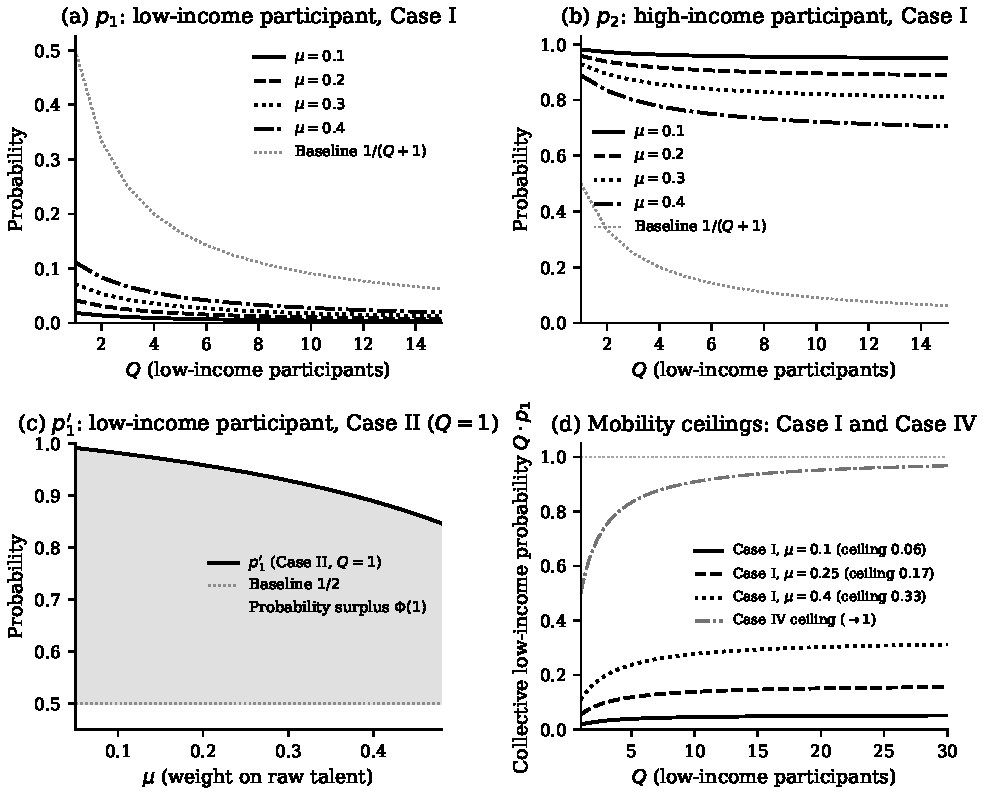
\includegraphics[width=5.5in]{winprob_main}
\par\end{centering}
\caption{\label{fig:Probability-of-winning}Winning probabilities and mobility
ceiling. $R=1$ high-income participant, $Q$ low-income participants. Dotted horizontal
lines in panels (a)--(b) show baselines $1/(Q+1)$ for each $Q$.}
\end{figure}

\subsubsection{Intertemporal Choice and Utility Payoffs}

Participants optimise an intertemporally additive utility $u(\cdot)$
over $T$ periods. In period 1 each participant decides whether to
pay $\overline{\nu}$; from period 2 onward she receives the income
corresponding to her position. Define the $T$-period discount sum
$D_{T}=\sum_{t=0}^{T-2}\delta^{-t}=(1-\delta^{-(T-1)})/(1-\delta^{-1})$,
where $\delta>1$ is the discount factor. The case $T=2$ gives $D_{T}=1$
and recovers the standard two-period model. The expected lifetime
utilities are:

\begin{align*}
\text{Low-income participant:} & \quad u(y_{1}-\nu_{1})+\frac{D_{T}}{\delta}\bigl[p_{1}^{c}\,u(y_{2})+(1-p_{1}^{c})\,u(y_{1})\bigr]\\
\text{High-income participant:} & \quad u(y_{2}-\nu_{2})+\frac{D_{T}}{\delta}\bigl[p_{2}^{c}\,u(y_{2})+(1-p_{2}^{c})\,u(y_{1})\bigr]
\end{align*}

where $p_{i}^{c}$ denotes the winning probability in case $c\in\{\mathrm{I,II,III,IV}\}$.
Define the utility costs of participation:

\begin{align*}
U_{1}\equiv u(y_{1})-u(y_{1}-\overline{\nu}),\qquad U_{2}\equiv u(y_{2})-u(y_{2}-\overline{\nu})
\end{align*}

Under diminishing marginal utility with $y_{1}<y_{2}$: $U_{2}<U_{1}$.
Table~\ref{tab:prisoners_dilemma_cases} summarises the four cases
as a $2\times2$ game, and Table~\ref{tab:prisoners_dilemma} reports
the utility payoffs.

\begin{table}[H]
\centering
\caption{\label{tab:prisoners_dilemma_cases}Investment strategies}
\smallskip
\begin{tabular}{lcc}
\toprule
 & \textit{Low-income withdraws} & \textit{Low-income invests}\\
\midrule
\textit{High-income withdraws} & Case III & Case II\\
\textit{High-income invests}   & Case I   & Case IV\\
\bottomrule
\end{tabular}
\end{table}

\begin{table}[H]
\centering
\caption{\label{tab:prisoners_dilemma}Utility payoffs (scale factor $D_{T}/\delta$
multiplies all second-period terms)}
\smallskip
\begin{tabular}{lll}
\toprule
 & \textit{Low-income withdraws} & \textit{Low-income invests}\\
\midrule
\textit{High-income withdraws} &
  $u(y_{2})+\dfrac{D_{T}}{\delta}\!\left[\tfrac{1}{Q+1}u(y_{2})+\tfrac{Q}{Q+1}u(y_{1})\right]$ \newline
  $u(y_{1})+\dfrac{D_{T}}{\delta}\!\left[\tfrac{1}{Q+1}u(y_{2})+\tfrac{Q}{Q+1}u(y_{1})\right]$
  &
  $u(y_{2})+\dfrac{D_{T}}{\delta}\!\left[(1-Qp_{1}')u(y_{2})+Qp_{1}'u(y_{1})\right]$ \newline
  $u(y_{1}-\overline{\nu})+\dfrac{D_{T}}{\delta}\!\left[p_{1}'u(y_{2})+(1-p_{1}')u(y_{1})\right]$
  \\[12pt]
\textit{High-income invests} &
  $u(y_{2}-\overline{\nu})+\dfrac{D_{T}}{\delta}\!\left[p_{2}u(y_{2})+(1-p_{2})u(y_{1})\right]$ \newline
  $u(y_{1})+\dfrac{D_{T}}{\delta}\!\left[p_{1}u(y_{2})+(1-p_{1})u(y_{1})\right]$
  &
  $u(y_{2}-\overline{\nu})+\dfrac{D_{T}}{\delta}\!\left[\tfrac{1}{Q+1}u(y_{2})+\tfrac{Q}{Q+1}u(y_{1})\right]$ \newline
  $u(y_{1}-\overline{\nu})+\dfrac{D_{T}}{\delta}\!\left[\tfrac{1}{Q+1}u(y_{2})+\tfrac{Q}{Q+1}u(y_{1})\right]$
  \\
\bottomrule
\end{tabular}
\begin{flushleft}
{\footnotesize In each cell: upper entry is high-income participant's utility;
lower entry is low-income participant's utility. $p_{1},p_{2}$ are Case~I
probabilities; $p_{1}'$ is the Case~II low-income-participant probability
($Q=1$ closed form; general $Q$ computed numerically). The high-income
participant's Case~II probability $1-Qp_{1}'$ satisfies
$1/(Q+1)-[1-Qp_{1}']=Q(p_{1}'-1/(Q+1))=Q\cdot\Phi(Q)/\text{scale}$,
valid for all $Q\geq1$.}
\end{flushleft}
\end{table}

\subsubsection{Nash Equilibrium Conditions}

For ease of notation define the probability-gap terms:

\begin{gather}
p_{1}\equiv\frac{\mu}{2(1-\mu)(Q+2)},\quad p_{2}\equiv1-Q\,p_{1}\nonumber\\
p_{1}'\equiv\frac{6-7\mu}{6(1-\mu)}\;(Q=1)\label{eq:probabilities}
\end{gather}

The ordering $p_{1}<1/(Q+1)<p_{2}$ and $p_{1}'>1/(Q+1)$
holds for all $\mu<1/2$ (Equation~\ref{eq:ordering}). Note that
$p_{2}'=1-Q\,p_{1}'$ satisfies $p_{2}'<1/(Q+1)$ by the same
ordering, but $p_{2}'$ does not appear in the equilibrium conditions
below: by the algebraic identity $1/(Q+1)-p_{2}'=Q(p_{1}'-1/(Q+1))$,
it is replaced throughout by $Q\cdot\Phi(Q)$, which is valid for all
$Q\geq1$.

\medskip
\noindent\textbf{Case I} (high-income invests, low-income withdraws) is a Nash
equilibrium if and only if:\footnote{Derived from: $u(y_{1})+\frac{D_{T}}{\delta}[p_{1}u(y_{2})+(1-p_{1})u(y_{1})]>u(y_{1}-\overline{\nu})+\frac{D_{T}}{\delta}[\frac{1}{Q+1}u(y_{2})+\frac{Q}{Q+1}u(y_{1})]$ for the low-income participant, and the reverse inequality for the high-income participant.}

\begin{gather}
\frac{D_{T}}{\delta}\left(\frac{1}{Q+1}-p_{1}\right)(u(y_{2})-u(y_{1}))<U_{1}\label{eq:caseI_poor}\\
U_{2}<\frac{D_{T}}{\delta}\left(p_{2}-\frac{1}{Q+1}\right)(u(y_{2})-u(y_{1}))\label{eq:caseI_rich}
\end{gather}

Both conditions hold simultaneously under diminishing utility since
$U_{2}<U_{1}$ and $p_{2}-1/(Q+1)\geq1/(Q+1)-p_{1}$. A higher
$\overline{\nu}$ favours Case~I so long as the high-income participant retains an incentive
to invest; a lower $\overline{\nu}$ can destabilise it if low-income
participants are induced to enter. Wider income differences ($y_{2}-y_{1}$
larger) reinforce the high-income participant's incentive to invest while
simultaneously raising the stakes enough to attract low-income investment,
making the first condition harder to satisfy.

\medskip
\noindent\textbf{Case II} (low-income invest, high-income withdraws). We now
state this case as a formal proposition, since it requires conditions
beyond standard diminishing utility and its characterisation carries
independent theoretical content.

\medskip
\noindent Define the probability surplus available to a low-income investor
when the high-income participant withdraws:
\begin{align}
\Phi(Q) & \equiv\frac{D_{T}}{\delta}\left(p_{1}'-\frac{1}{Q+1}\right)(u(y_{2})-u(y_{1}))\label{eq:Phi_def}
\end{align}

Since $p_{1}'>1/(Q+1)$ for all $\mu<1/2$ (Equation~\ref{eq:ordering}),
$\Phi(Q)>0$ always. For $Q=1$, substituting
$p_{1}'=(6-7\mu)/[6(1-\mu)]$ yields:
\begin{align}
\Phi(1) & =\frac{D_{T}}{\delta}\cdot\frac{3-4\mu}{6(1-\mu)}\cdot(u(y_{2})-u(y_{1}))\label{eq:Phi_Q1}
\end{align}

where $(3-4\mu)>0$ for all $\mu<1/2$ under Assumption~\ref{assu:mu_less_than_half},
so $\Phi(1)$ is strictly positive and decreasing in $\mu$. For
$Q\geq2$, $p_{1}'$ has no single closed form across general $Q$
(as noted in Section~\ref{subsec:Two-player-Discrete-Model}), but
$\Phi(Q)$ is computable numerically for any $(Q,\mu)$ and inherits
the ordering $\Phi(Q)>0$ for all $\mu<1/2$. The qualitative
conclusions of Proposition~\ref{prop:caseII} --- that Case~II
requires reference-dependent preferences for all $Q\geq1$ and that
the feasibility window $[U_1, U_2/Q]$ narrows as $\mu$ increases
--- hold for general $Q$ by the ordering results in
Equation~\ref{eq:ordering}.

\begin{proposition}[Case II Nash Equilibrium]\label{prop:caseII}
Case II (low-income invest, high-income withdraws) is a Nash equilibrium if and
only if:
\begin{gather}
U_{1}<\Phi(Q)\leq U_{2}/Q\label{eq:caseII_NSC}
\end{gather}
A necessary condition is therefore $Q\cdot U_{1}<U_{2}$. Under
standard diminishing utility with $y_{1}<y_{2}$, $U_{2}<U_{1}$,
so $U_{2}/Q<U_{1}$ for all $Q\geq1$ and Condition~\eqref{eq:caseII_NSC}
cannot be satisfied. Case II requires reference-dependent preferences
under which $U_{1}<U_{2}$ --- the marginal utility cost of $\overline{\nu}$
is higher for the low-income participant than for the high-income participant, reversing the
standard concavity ordering. For $Q=1$, the condition reduces to:
\begin{align}
U_{1}<\Phi(1)\leq U_{2}\label{eq:caseII_Q1}
\end{align}
which is feasible if and only if $U_{1}<U_{2}$.
\end{proposition}

\begin{proof}
Condition~\eqref{eq:caseII_NSC} is derived directly from the utility
payoffs in Table~\ref{tab:prisoners_dilemma}. The low-income participant
prefers to invest given the high-income participant withdraws if and only if
$U_{1}<\Phi(Q)$. The high-income participant prefers to withdraw given the
low-income participants invest if and only if the gain from deviating to investment,
$\frac{D_{T}}{\delta}(1/(Q+1)-p_{2}')(u(y_{2})-u(y_{1}))=Q\cdot\Phi(Q)$
(using $1/(Q+1)-p_{2}'=Q(p_{1}'-1/(Q+1))$, valid for all $Q\geq1$),
is less than the cost $U_{2}$, i.e. $U_{2}\geq Q\cdot\Phi(Q)$,
equivalently $\Phi(Q)\leq U_{2}/Q$. Both conditions together require
$U_{1}<U_{2}/Q$. Under standard concavity $U_{2}<U_{1}$, so
$U_{2}/Q<U_{1}$ for all $Q\geq1$ and the condition fails. $\square$
\end{proof}

\medskip

Several features of this proposition deserve comment. First,
$\Phi(1)$ is strictly decreasing in $\mu$: as social capital is
weighted more heavily, the probability surplus from being the sole
investor narrows, and the Case~II window must be correspondingly
tighter to sustain the equilibrium. At $\mu\to0$ (pure raw-talent
competition), $\Phi(1)\to1/2$, giving the widest possible window;
at $\mu\to1/2$ (Assumption~\ref{assu:mu_less_than_half} binding),
$\Phi(1)\to1/3$. Second, the equilibrium remains fragile even when
it exists: higher $\overline{\nu}$, greater impatience ($\delta$
rising), or wider income differences ($y_{2}-y_{1}$ larger) can each
collapse it into Case~III or Case~IV respectively
\cite{MijsMeritocracy2020,MijsParadox2019}.

\medskip
\noindent\textbf{Case III} (neither invests) is a Nash equilibrium if:\footnote{Both participants prefer withdrawal given the other withdraws.}

\begin{gather*}
U_{1}>\frac{D_{T}}{\delta}\left(p_{1}'-\frac{1}{Q+1}\right)(u(y_{2})-u(y_{1}))\\
U_{2}>\frac{D_{T}}{\delta}\left(p_{2}-\frac{1}{Q+1}\right)(u(y_{2})-u(y_{1}))
\end{gather*}

Since $p_{1}'-1/(Q+1)\leq p_{2}-1/(Q+1)$ and $U_{2}<U_{1}$, the
binding constraint is the second inequality. Case~III prevails when
participation costs are prohibitively high relative to the income
gain. If there is any net utility from competition, Case~IV is the
likely outcome.

\medskip
\noindent\textbf{Case IV} (both invest) is a Nash equilibrium if:\footnote{Both participants prefer investment given the other invests.}

\begin{gather}
U_{1}<\frac{D_{T}}{\delta}\left(\frac{1}{Q+1}-p_{1}\right)(u(y_{2})-u(y_{1}))\label{eq:caseIV_poor}\\
U_{2}<Q\cdot\Phi(Q)\label{eq:caseIV_rich}
\end{gather}

With $U_{2}<U_{1}$, this equilibrium rests on the low-income participant's
incentive: so long as the low-income participant finds the competition
worthwhile, the high-income participant also participates. Note that
Equations~\ref{eq:caseI_poor} and~\ref{eq:caseIV_poor} are exact
complements --- Case~IV obtains precisely where Case~I fails for
the low-income participant. The high-income participant's condition
$U_{2}<Q\cdot\Phi(Q)$ uses the algebraic identity
$1/(Q+1)-p_{2}'=Q(p_{1}'-1/(Q+1))$, which holds for all $Q\geq1$
and connects Case~IV directly to the probability surplus $\Phi(Q)$
from Proposition~\ref{prop:caseII}: the high-income participant's boundary
between Cases~II and~IV is exactly $Q\cdot\Phi(Q)$.

\medskip

These conditions confirm that under diminishing utility only Cases~I
and~IV are generically stable. For very low $\overline{\nu}$, both
participants invest (Case~IV); for very high $\overline{\nu}$, only
the high-income participant invests (Case~I); for sufficiently extreme $\overline{\nu}$,
neither invests (Case~III). Case~II requires a non-standard utility
structure and remains fragile throughout.

\subsubsection{\label{subsec:Threshold}Participation Threshold}

The boundary between Cases~IV and~I is defined by the critical
cost $\overline{\nu}^{*}$ at which the low-income participant is indifferent
between investing and withdrawing, given the high-income participant invests.
Setting Equation~\ref{eq:caseIV_poor} as an equality:

\begin{align}
u(y_{1})-u(y_{1}-\overline{\nu}^{*}) & =\frac{D_{T}}{\delta}\left(\frac{1}{Q+1}-p_{1}\right)(u(y_{2})-u(y_{1}))\label{eq:threshold_general}
\end{align}

The qualitative properties of $\overline{\nu}^{*}$ --- that it is
interior, positive, decreasing in $Q$, and decreasing in $\mu$ ---
follow from the general condition~\eqref{eq:threshold_general} for
any strictly increasing concave $u(\cdot)$. Log utility provides a
tractable closed form for illustration:

Under log utility $u(y)=\log(y)$, this yields:

\begin{align}
\overline{\nu}^{*} & =y_{1}\left(1-\left(\frac{y_{1}}{y_{2}}\right)^{A}\right),\qquad
A=\frac{D_{T}}{\delta}\left(\frac{1}{Q+1}-\frac{\mu}{2(1-\mu)(Q+2)}\right)\label{eq:nu_star}
\end{align}

Since $1/(Q+1)>p_{1}$ for all $\mu<1/2$ (Equation~\ref{eq:ordering}),
we have $A>0$ and hence $\overline{\nu}^{*}\in(0,y_{1})$: the
threshold is always interior and affordable by the low-income participant.
For $T=2$ ($D_{T}=1$), $A$ reduces to $(1/\delta)(1/(Q+1)-p_{1})$.
The T-period generalisation is detailed in Appendix~\ref{sec:appendix_Tperiod}.

\subsubsection{\label{subsec:Comparative-Statics}Comparative Statics}

The participation window --- the set of $\overline{\nu}$ values
that sustain Case~IV --- is determined by $A$ in Equation~\ref{eq:nu_star}.
Two comparative statics follow directly from the closed-form expression
for $A$:

\medskip
\noindent\textbf{Credential inflation} ($\mu$ decreasing, social
capital weighted more heavily):

\begin{align}
\frac{\partial A}{\partial\mu} & =-\frac{1}{2(Q+2)(1-\mu)^{2}}<0\label{eq:dA_dmu}
\end{align}

The sign is negative for all admissible $\mu\in(0,1/2)$ and all
$Q\geq1$: as social capital becomes more decisive relative to raw
talent, $A$ decreases and $\overline{\nu}^{*}$ falls. The economic
mechanism is direct. When $\mu$ is low, the informational advantage
of investing in social capital is large --- a low-income participant who
pays $\overline{\nu}$ gains substantially more than a non-investor
--- so the participation window is wide. As $\mu\to0$ (pure social
capital competition), $A\to1/(Q+1)$, the window is at its maximum.
As $\mu$ rises toward $1/2$ (Assumption~\ref{assu:mu_less_than_half}
binding), $A\to(Q+3)/[2(Q+1)(Q+2)]$, which is still positive but
substantially reduced. The implication is that credential inflation
--- institutional credentials becoming more decisive relative to
innate ability, which is the empirically relevant direction in elite
labour markets --- closes the range of costs that sustain universal
participation. Low-income participants are priced out not because costs
rise but because the informational return to investing falls as
social capital becomes near-universal among competitors.

\medskip
\noindent\textbf{Competition size} ($Q$ increasing, more low-income challengers):

\begin{align}
\frac{\partial A}{\partial Q} & =\frac{-\mu(Q+1)^{2}+2(1-\mu)(Q+2)^{2}}{2(Q+1)^{2}(Q+2)^{2}(1-\mu)}\cdot\frac{1}{\delta}\label{eq:dA_dQ}
\end{align}

Since $\mu<1$, the denominator
$2(Q+1)^{2}(Q+2)^{2}(\mu-1)<0$, while the numerator
$N=2(1-\mu)(Q+2)^{2}-\mu(Q+1)^{2}$ satisfies $N>(Q+2)^{2}-\tfrac{1}{2}(Q+1)^{2}=\tfrac{1}{2}Q^{2}+3Q+\tfrac{7}{2}>0$
for all $Q\geq0$ under $\mu<\tfrac{1}{2}$. Hence $\partial A/\partial Q<0$.
As the pool of low-income challengers grows, $A$ decreases and
$\overline{\nu}^{*}$ falls. Equivalently, a larger $Q$ makes Case~I
increasingly likely to prevail over Case~IV. As $Q\to\infty$, $A\to0$
and the participation window closes entirely.

\medskip
\noindent\textbf{Competition size and real-world competition structures.}
The comparative statics on $Q$ and $\mu$ map onto an observable
empirical distinction between small and large competitions.

In small competitions --- partner-track interviews at professional
firms, senior academic appointments, board-level selections --- the
field of challengers is narrow and assessors can observe social
capital directly: cultural fit, network affiliation, institutional
credentials and communication style are all legible at close range.
This corresponds to low $\mu$ (social capital decisive) and low $Q$.
The model implies that in this regime the participation window $A$ is
relatively wide, both Cases~I and~IV are plausible depending on cost
levels, and the mobility ceiling $\mu/[2(1-\mu)]$ is already binding
in proportional terms. Individual low-income participants have non-negligible
probabilities, yet class-level mobility is sharply constrained by $\mu$.
Case~II is also most plausible here: the fragile equilibrium in which
only the low-income participants over-invest in credentials --- consistent with the
sociological observation that aspiring candidates from lower-income
backgrounds disproportionately invest in elite signals in highly
selective, socially-embedded competitions
\cite{HeckmanMosso2014,MijsParadox2019}.

In large competitions --- national civil service examinations, mass
graduate recruitment schemes, standardised professional qualifications
--- the field is wide and assessors cannot observe social capital
individually. Standardisation is typically designed to increase the
weight on raw talent, i.e. to raise $\mu$. The model implies two
simultaneous effects. First, $\partial A/\partial Q<0$ means the
participation window closes as the field grows: the range of costs
supporting universal participation shrinks, pushing toward elite-only
equilibria regardless of intent. Second, raising $\mu$ through
standardised assessment increases the ceiling $\mu/[2(1-\mu)]$ and
can partially offset this window-closing effect. The model thus
provides a formal basis for the policy intuition that the \emph{design}
of large competitions --- what they test, how accessible they are ---
matters more for class-level mobility than the design of small ones:
in large competitions, the $\mu$-effect on the ceiling and the
$Q$-effect on the participation window are the two levers, and they
must be managed jointly.

\subsubsection{\label{subsec:Mobility-Ceiling}Collective Low-Income Probability
and the Mobility Ceiling}

The analysis so far has focused on the per-low-income-participant winning
probability $p_{1}$. A distinct and complementary object is the
\emph{collective low-income probability} $Q\cdot p_{1}$, which measures
the probability that any low-income participant displaces the high-income participant --- a
statement about class-level mobility rather than individual opportunity.
Two ceilings emerge depending on which equilibrium prevails.

\medskip
\noindent\textbf{Case I ceiling.} Under Case~I, the collective low-income
probability in closed form is:

\begin{align}
Q\cdot p_{1} & =\frac{Q\mu}{2(1-\mu)(Q+2)}\label{eq:collective}
\end{align}

As $Q\to\infty$:

\begin{align}
\lim_{Q\to\infty}Q\cdot p_{1} & =\frac{\mu}{2(1-\mu)}\label{eq:ceiling}
\end{align}

This ceiling is bounded strictly below $\tfrac{1}{2}$ for all
$\mu<\tfrac{1}{2}$ and is increasing in $\mu$.

\medskip
\noindent\textbf{Case IV ceiling.} Under Case~IV (both invest),
all $Q+1$ participants draw from the same distribution $F_{X}$, so
$p_{1}=1/(Q+1)$ and:

\begin{align}
\lim_{Q\to\infty}Q\cdot\frac{1}{Q+1} & =1\label{eq:ceiling_IV}
\end{align}

Under universal participation, collective low-income mobility approaches
certainty as the field grows.

\medskip
\noindent\textbf{Why the Case~I ceiling is the economically relevant
one.} The two ceilings appear to give contradictory messages about
the social limits to growth. The resolution lies in the comparative
statics: by Equation~\ref{eq:dA_dQ}, $\partial A/\partial Q<0$, so
a larger pool of low-income challengers \emph{tightens} the participation
window and makes Case~I increasingly likely to prevail over Case~IV.
The Case~I ceiling is therefore precisely the one that binds as $Q$
grows: the equilibrium converges toward elite-only participation at
exactly the same rate as collective mobility approaches its hard
limit. The Case~IV ceiling ($\to1$) is relevant only when $Q$ is
small and costs are low enough to sustain universal participation ---
the regime where mobility concerns are least acute. It is the Case~I
ceiling $\mu/[2(1-\mu)]$ that constitutes the binding social limit
to growth in the sense of \citeA{HirschSocialLimits}.

Simultaneously, the \emph{individual} low-income participant's probability
$p_{1}\to0$ as $Q\to\infty$: each low-income participant's chances vanish
even as collective mobility converges to the ceiling. This divergence
between individual and collective mobility --- the many trying, the
class ceiling binding --- is the formal content of the social limits
argument.

\section{\label{sec:Conclusion}Conclusion}

\noindent

This paper develops a formal model of status competition to clarify
the conditions under which a persistent empirical tension arises.
Post-war scholars predicted that narrowing income gaps would intensify
positional rivalry; empirical research consistently finds the opposite.
We show that this tension is tractable once participation in status
competitions is treated as an endogenous equilibrium outcome shaped
by the joint configuration of income differences and participation
costs --- and that the empirical pattern is the generic case under
our model's assumptions.

The model fixes one high-income participant against a variable pool of $Q$
low-income challengers competing through probabilistic tournaments that
combine innate ability and acquired social capital. By deriving
participation decisions from intertemporal utility maximisation over
$T$ periods, we obtain four principal results. First, under diminishing
wealth utility, only two stable Nash equilibria exist: universal
participation, in which both high-income and low-income participants invest in social capital,
and elite-only participation, in which only the high-income participant does. This binary
structure formalises Hirsch's (\citeyear{HirschSocialLimits}) social
limits to growth as an equilibrium theorem rather than a qualitative
conjecture. Second, the transition between these equilibria is governed
by a participation threshold $\overline{\nu}^{*}=y_{1}(1-(y_{1}/y_{2})^{A})$,
where $A$ decreases in both competition intensity $Q$ and credential
inflation ($\mu$ falling). Wider inequality sustains high-income investment
even as it prices out low-income participants, explaining why status expenditure
and inequality can rise together. Third, reference-dependent utility introduces a
boundary equilibrium --- characterised by a formal proposition --- in
which only the low-income participants invest, requiring $U_{1}<U_{2}$ and a feasibility
window that narrows as social capital is weighted more heavily. Fourth,
individual low-income mobility probability vanishes as $Q\to\infty$, but
collective class-level mobility converges to $\mu/[2(1-\mu)]$ under
Case~I and to $1$ under Case~IV. The Case~I ceiling is the binding
one: the comparative statics on $Q$ drive the equilibrium toward
elite-only participation at exactly the rate that collective mobility
approaches this hard limit. It is therefore the Case~I ceiling ---
not the trivial Case~IV limit --- that constitutes the operative
social limit to growth in the empirically relevant regime.

For the analysis of inequality and status competition, the results
clarify that reducing income differences without simultaneously
lowering participation costs may leave elite-only equilibria intact.
Conversely, policies that lower the threshold cost $\overline{\nu}$
--- through subsidies to credential acquisition, reduced network
barriers, or open-access professional qualifications --- expand
$\overline{\nu}^{*}$ and can restore the universal participation
equilibrium. The mobility ceiling $\mu/[2(1-\mu)]$ further implies
that in competitions where institutional affiliation and credentials
dominate raw ability, no amount of low-income participation alone can
overcome the structural investment advantage of the high-income participant. Increasing
$\mu$ --- making raw talent more decisive relative to social capital
--- is therefore a necessary complement to cost-reduction policies
if class-level mobility is to exceed the ceiling.

Several assumptions bound the analysis and point to natural
extensions. The model fixes $R=1$ throughout; with $R>1$ high-income
participants the binary equilibrium structure is preserved but the
mobility ceiling becomes $R\cdot\mu/[2(1-\mu)(R+1)]$, approaching
the same limit as $R\to\infty$ normalised by population share.
The threshold cost structure is binary --- pay $\overline{\nu}$ in
full or not at all --- which generates the clean closed-form results
but abstracts from continuous investment intensities; a convex cost
function would smooth the participation boundary and generate richer
comparative statics on the income distribution. Most substantively,
the incomes $y_1$ and $y_2$ are exogenous: the model identifies how
inequality shapes participation given a distribution of positions,
but not how status competition feeds back into the income distribution
over time. Integrating the participation mechanism with an endogenous
income process --- closer in spirit to \citeA{ColeMailaithPostlewaite1992}
--- would allow the model to speak to the long-run co-evolution of
inequality and credential investment, which the empirical literature
increasingly documents \cite{MijsParadox2019,MijsMeritocracy2020}.

\bibliographystyle{apacite}
\bibliography{status_consumption}

\begin{appendices}
\section{Convolution of Uniform Random Variables} \label{sec:appendix_theoretical_1}

The distribution of a convex combination $w=\mu r+(1-\mu)s$ of two
random variables $r,s$ - which are distributed according to densities
$f_{R}(r)$ and $f_{S}(s)$ - can be derived using the convolution
of two derived variables $x=\mu r$ and $y=(1-\mu)s$. If $r$ and
$s$ are uniformly distributed variables ranging from 0 to 1, then
$x$ ranges from 0 to $\mu$ and $y$ ranges from $0$ to $(1-\mu)$.
The CDF for $F_{X}(x)$ and $F_{Y}(y)$ are simply $F_{X}(x)=\frac{x}{\mu}$
, $F_{Y}(y)=\frac{y}{1-\mu}$ (respectively). Therefore, the densities
for $x$ and $y$ are $f_{X}(x)=\frac{1}{\mu}$ and $f_{Y}(y)=\frac{1}{1-\mu}$.
The density of $w$ is simple $f(w)=\int_{-\infty}^{\infty}f_{Y}(w-x)f_{X}(x)dx$.
Since , $f_{X}(x)$ is $1/\mu$ only between $0$ and $\mu$. We have
the following integral to evaluate for the convolution

\begin{align*}
f(w) & =\frac{1}{\mu}\int_{0}^{\mu}f_{Y}(w-x)dx
\end{align*}

Since $f_{Y}(y)$ is 1 only between 0 and $1-\mu$, we have the condition
$0<w-x<1-\mu\Rightarrow w-(1-\mu)<x<w$. Further, $x$ is distributed
only between 0 and $\mu$. As shown in Figure \ref{fig:convex_combo},
the integral would evaluate to the following\footnote{Notice that as a convex combination, $w$ is distributed only between
0 and 1.} under the assumption $\mu<\frac{1}{2}$.

\begin{align*}
f(w)=\frac{1}{\mu}\int_{0}^{\mu}f_{Y}(w-x)dx & =\begin{cases}
\frac{1}{\mu}\int_{0}^{w}\frac{1}{1-\mu}dx & 0<w<\mu\\
\frac{1}{\mu}\int_{0}^{\mu}\frac{1}{1-\mu}dx & \mu<w<1-\mu\\
\frac{1}{\mu}\int_{w-(1-\mu)}^{\mu}\frac{1}{1-\mu}dx & 1-\mu<w<1\\
0 & \text{otherwise}
\end{cases}
\end{align*}

This can be simplified as 

\begin{align*}
f(w) & =\begin{cases}
\frac{w}{\mu(1-\mu)} & 0<w<\mu\\
\frac{1}{1-\mu} & \mu<w<1-\mu\\
\frac{1-w}{\mu(1-\mu)} & 1-\mu<w<1\\
0 & \text{otherwise}
\end{cases}
\end{align*}

Figure \ref{fig:convex_combo_plot} shows this trapezoidal density
with $\mu$ set to $\frac{1}{5}$. The CDF $F_{X}(x)$ can be evaluated
by integrating the above density as $P(X<x)=\int_{-\infty}^{x}f(t)dt$. 

\begin{align*}
F_{X}(x) & =\begin{cases}
\frac{x^{2}}{2\mu(1-\mu)} & 0<x<\mu\\
\frac{\mu}{2(1-\mu)}+\frac{x-\mu}{1-\mu} & \mu<x<1-\mu\\
\frac{\mu^{2}}{2\mu(1-\mu)}+\frac{2\mu(1-2\mu)}{2\mu(1-\mu)}+\frac{\mu^{2}-x^{2}+2x-1}{2\mu(1-\mu)} & 1-\mu<x<1\\
0 & \text{otherwise}
\end{cases}
\end{align*}

Simplifying above, we have

\begin{align*}
F_{X}(x) & =\begin{cases}
\frac{x^{2}}{2\mu(1-\mu)} & 0<x<\mu\\
\frac{x-\mu/2}{1-\mu} & \mu<x<1-\mu\\
1-\frac{(x-1)^{2}}{2\mu(1-\mu)} & 1-\mu<x<1\\
0 & \text{otherwise}
\end{cases}
\end{align*}

\begin{figure}[H]
\begin{centering}
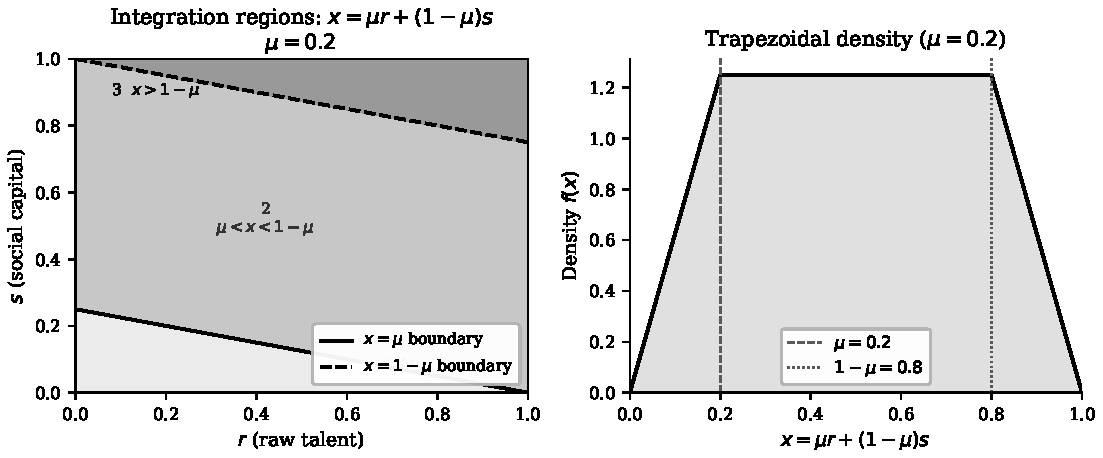
\includegraphics[width=5in]{density_appendix}
\par\end{centering}
\caption{\label{fig:convex_combo}Left: ranges of $w$ and $x$ for convolution
of two scaled random variables. Right: trapezoidal density of $w$
as the convex combination with $\mu=\frac{1}{5}$.}
\end{figure}

\newpage
\section{$P(\text{win}|r,s)$} \label{sec:appendix_theoretical_2} 

To calculate $\int_{s=0}^{s=1}\int_{r=0}^{r=1}P(\text{win}|r,s)drds$
over the variable $x$ (where $0<r<1$ and $0<s<1$), we evaluate
the sum of three parts split by the boundaries of the piecewise function.
The three parts are shown in Figure \ref{fig:integral_boundaries}.
If $x=\mu r+(1-\mu)s$ and $F(x)$ is of the following piece-wise
form

\begin{align*}
F(x) & =\begin{cases}
A & 0<x<\mu\\
B & \mu<x<1-\mu\\
C & 1-\mu<x<1\\
0 & \text{otherwise}
\end{cases}
\end{align*}

Then the integral $\int_{s=0}^{s=1}\int_{r=0}^{r=1}F(x)drds$ can
be written as

\begin{align*}
\int_{s=0}^{s=1}\int_{r=0}^{r=1}F(x)dsdr & =\int_{r=0}^{r=1}{\int_{s=0}^{s=\frac{\mu(1-r)}{1-\mu}}A\ dsdr}+\int_{r=0}^{r=1}{\int_{s=\frac{\mu(1-r)}{1-\mu}}^{s=1-\frac{\mu r}{1-\mu}}B\ dsdr}+\int_{r=0}^{r=1}{\int_{s=1-\frac{\mu r}{1-\mu}}^{s=1}C\ dsdr}
\end{align*}

\begin{figure}[H]
\begin{centering}
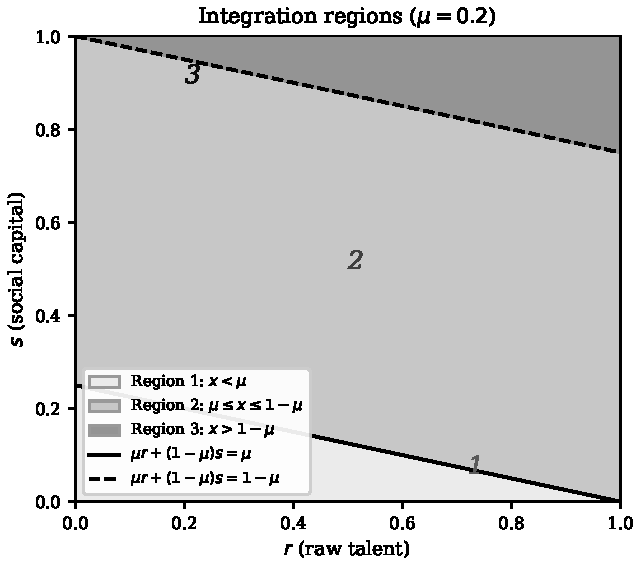
\includegraphics[width=4in]{integral_regions}
\par\end{centering}
\caption{\label{fig:integral_boundaries}Integration over $r,s$ split by boundaries
$\mu r+(1-\mu)s=\mu$ and $\mu r+(1-\mu)s=1-\mu$}
\end{figure}

\newpage
\section{T-Period Utility Generalisation}\label{sec:appendix_Tperiod}

The main text presents intertemporal utility under $T$ periods with
discount sum $D_{T}=\sum_{t=0}^{T-2}\delta^{-t}$. We establish
here that the qualitative equilibrium structure is unchanged by $T$.

\medskip
\noindent\textbf{Closed form for $D_{T}$.} Since $\delta>1$, the
geometric sum evaluates to:
\[
D_{T}=\frac{1-\delta^{-(T-1)}}{1-\delta^{-1}}
\]
For $T=2$: $D_{T}=1$, recovering the two-period model. For $T=3$:
$D_{T}=1+1/\delta$.

\medskip
\noindent\textbf{Proposition (T-period invariance).} \textit{The
set of Nash equilibria under $T$-period utility is identical to
that under two-period utility ($T=2$). The participation threshold
$\overline{\nu}^{*}$ scales monotonically with $D_{T}$: it is
strictly increasing in $T$ and strictly decreasing in $\delta$.}

\medskip
\noindent\textit{Proof.} All Nash equilibrium conditions (Equations
\ref{eq:caseI_poor}--\ref{eq:caseIV_rich}) share the structure:
\[
\frac{D_{T}}{\delta}\cdot\Delta p\cdot(u(y_{2})-u(y_{1}))\gtrless U_{i}
\]
where $\Delta p$ is a probability gap and $U_{i}$ is a utility
cost. Since $D_{T}/\delta$ is a common positive scaling factor,
it does not alter which side of any inequality is larger: an equilibrium
condition satisfied under $T=2$ is satisfied for all $T\geq2$ with
the same qualitative direction. The threshold $\overline{\nu}^{*}$
(Equation~\ref{eq:nu_star}) has $A\propto D_{T}/\delta$; since
$(y_{1}/y_{2})^{A}$ is decreasing in $A$ and $y_{1}<y_{2}$,
$\overline{\nu}^{*}=y_{1}(1-(y_{1}/y_{2})^{A})$ increases with
$A$, hence with $D_{T}$. $D_{T}$ is strictly increasing in $T$
(adding positive terms) and strictly decreasing in $\delta$ (each
term $\delta^{-t}$ is decreasing in $\delta$). $\square$

\medskip
The proposition implies that a longer investment horizon or greater
patience raises $\overline{\nu}^{*}$, expanding the range of costs
under which universal participation (Case~IV) is sustained. The
two-period model is therefore a conservative baseline: all comparative
statics on $\overline{\nu}^{*}$ with respect to $\mu$ and $Q$
carry over unchanged to the $T$-period case.

\end{appendices}
\end{document}
